\documentclass[]{interact}
\usepackage{epstopdf}% To incorporate .eps illustrations using PDFLaTeX, etc.
\usepackage{subfigure}% Support for small, `sub' figures and tables
%\usepackage[nolists,tablesfirst]{endfloat}% To `separate' figures and tables from text if required

\usepackage{natbib}
\bibliographystyle{chicago}
\setcitestyle{authoryear,open={(},close={)}}
\renewcommand\bibfont{\fontsize{10}{12}\selectfont}% Bibliography support using natbib.sty

\usepackage{hyperref}
\hypersetup{
    colorlinks=true,
    linkcolor=blue,
    filecolor=magenta,
    urlcolor=blue,
    citecolor=blue,
}

\usepackage{titlesec}
\titleformat*{\section}{\Large\bfseries}
\titleformat*{\subsection}{\large\bfseries}

\usepackage{endnotes}
\let\footnote=\endnote
\usepackage{etoolbox}
\patchcmd{\enoteformat}{1.8em}{0pt}{}{}

\theoremstyle{plain}% Theorem-like structures provided by amsthm.sty
\newtheorem{theorem}{Theorem}[section]
\newtheorem{lemma}[theorem]{Lemma}
\newtheorem{corollary}[theorem]{Corollary}
\newtheorem{proposition}[theorem]{Proposition}

\theoremstyle{definition}
\newtheorem{definition}[theorem]{Definition}
\newtheorem{example}[theorem]{Example}

\theoremstyle{remark}
\newtheorem{remark}{Remark}
\newtheorem{notation}{Notation}

\usepackage{tabularx}
\usepackage{booktabs,caption}
\usepackage{threeparttable}

\usepackage{lscape}
%%%%%%%%%%%%%%%%%%%%%%%%%%%%%%%%%%%%%%%%%%%%%%%%%%

\begin{document}

\articletype{DRAFT MANUSCRIPT}

\title{Replication Survey}

\author{
\name{Peter Kedron\textsuperscript{a,b}\thanks{CONTACT Peter Kedron. Email: Peter.Kedron@asu.edu}, Joseph Holler\textsuperscript{c}, and Sarah Bardin\textsuperscript{a,b}}
\affil{\textsuperscript{a}School of Geographical Sciences and Urban Planning, Arizona State University, Tempe, Arizona, USA; \textsuperscript{b}Spatial Analysis Research Center (SPARC), Arizona State University, Tempe, Arizona, USA; \textsuperscript{c}Department of Geography, Middlebury College, Middlebury, Vermont, USA}
}

\maketitle

\begin{abstract}
Write Abstract

\end{abstract}

\begin{keywords}
Reproducible Research, Epistemology, Geographic Research Methods
\end{keywords}

%%%%%%%%%%%%%%%%%%%%%%%%%%%%%%%%%%%%%%%%%%%%%%%%%%
\newpage
\section*{Introduction}
Since the 1600s, replication has been a defining characteristic of the scientific method and an essential tool of researchers working to remove errors from our understanding of phenomena. 
\citet{nosek2020} broadly define a replication as any study that has at least one outcome that would be considered to be diagnostic evidence of a claim from prior research.
More frequently, replication is defined along two axes that help to distinguish the type of diagnostic evidence a study will provide and the function or purpose it is intended to serve. 
First, it is common to distinguish whether a replication study used the same data as the original study, or if new data were collected and analyzed. 
Second, it is helpful to identify whether a replication is focused on the question of whether the specific results of the original study can be reobserved, or whether the conclusions drawn from the original study are robust to changes in procedure or context.

When a researcher asks whether the same data and procedures can be used to generate the same results as an original study the central purpose of their study is verification.
If the researcher uses the original data, but introduces procedural differences they think may effect the original result they pursue a reanalysis designed to determine whether the original reasoning was somehow erroneous. 
Both of these approaches to replication assess the internal validity of research and are more commonly referred to as reproductions.
If the researcher tries to follow the procedures of an original study, but collects new data, the purpose shifts to evaluating the external validity of the original result by retesting it under new conditions.
This approach is commonly referred to as replication. 

While a replication or reproduction can never provide conclusive evidence for or against a finding, either type of study can be informative. 
If a well-executed, high-quality replication or reproduction recreates the result of an original study, we are apt to increase our confidence in the original findings. 
If a finding cannot be recreated, it reduces our confidence in the original result and suggests that our current understanding of the system being studied or our methods of testing that system are insufficient.

For example, in a survey of 807 ecologists and evolutionary biologists, 64 percent admitted to failing to report non-significant results and 51 percent admitted to presenting unexpected findings as if they had been hypothesized from the start of the research \citep{fraser2018questionable}.

%%%%%%%%%%%%%%%%%%%%%%%%%%%%%%%%%%%%%%%%%%%%%%%%%%
\section*{Results}

%%%%%%%%%%%%%%%%%%%%%%%%
\subsection*{Survey Response Demographics}
A total of \textit{n}=283 of the authors we contacted completed the online survey with information sufficient for analysis. 
The contact rate for the survey was 17.7 percent, the response rate was 11.3 percent, yielding a cooperation rate of 64.0 percent. 
The refusal rate was 6.4 percent\endnote{All outcome rates are reported using \citet{aaporstandards} standards. 
The outcome rates used were - response rate 2, cooperation rate 2, refusal rate 1, and contact rate 1.}.
Respondents were predominantly male (65.1\%) and between the ages of 35 and 55 (62.4\%). 
The majority of respondents were also academics, but were well balanced across career levels as no one category made up more that 30 percent of the sample.
Respondents were similarly balanced across disciplinary subfields, but did contain a greater number of physical geographers  - human geography (26.8\%), physical geography (39.9\%), nature and society (14.8\%), geographic methods and GIScience (17.3\%). 
Different methodological approaches were well represented by respondents in the sample with qualitative researchers making up the smallest sub-group  - quantitative (47.3\%), qualitative (16.3\%), and mixed-methods (36.0\%).

%%%%%%%%%%%%%%%%%%%%%%%%
\subsection*{Researcher Definitions of Replication and its Epistemic Functions}
\begin{itemize}
    \item Respondents report thinking about replicability (73.9\%) talking with colleagues about replicability (65.0\%) and considering replicability when undertaking peer-review (59.0\%). 
    \item Far fewer respondents report attempting replications (31.8\%). 
\end{itemize}

\begin{itemize}
    \item Coded analysis of Q6
\end{itemize}

A majority of respondents believe replications can serve epistemic functions.
\begin{itemize}
    \item Q7 control of chance 64.5\%
    \item Q7 identify product of flawed design 59.7\%
    \item Q7 construct validity 75.2\%
    \item External validity population 62.9\%
    \item External validity location 67.8\%
    \item Human, Nature Society, and Qualitative researchers had lower agreement on each point.
\end{itemize}

%%%%%%%%%%%%%%%%%%%%%%%%
\subsection*{Replication - Chances and motivations}
Overall geographic researchers believe that the majority of research in the discipline has not been independently replicated and appear to be uncertain about what proportion of literature could or should be replicated (Figure \ref{fig:Q12-HCS}). 
On average, respondents estimated that 25 percent of recent studies in their sub-field have be replicated. 
However, this average likely overstates the percentage of studies researchers believe have been replicated because the response distribution is strongly right skewed.
Our median response to this question is 20 percent and a heavy tail of containing 46.9 percent of responses estimated that less than 10 percent of recent studies have been replicated.
On average, respondents estimated that approximately half of studies 'could be replicated' (55.0\%) or 'should be replicated' (55.9\%). 
However, these averages are the product of the relatively flat distributions of estimates across the range of possible values. 
The response to both questions was also highly variable (\textit{$sd_{could}=24.3\%$}, \textit{$sd_{should}=27.7\%$}) indicating no common knowledge or belief about the possibility or value of replicating recent work.  

\begin{center}
\textbf{Insert Figure \ref{fig:Q12-HCS} About Here}
\end{center}

Q8-11 Factors that affect the chances of replicating a claim.
Researchers collectively indicated that only a few study characteristics of phenomenon characteristics would alter an independent researcher's chances of replicating a prior claim. 
Researcher identified more study characteristics than phenomena characteristics, which may indicate they they are thinking of this through the lens of artifact availability from the prior study and not the nature of the phenomena. 
A small but notable percentage of researchers indicated that they simply did not know whether a factor would affect chances of replication. 


Only a subset of study characteristics were consistently identified by geographic researchers as altering the chances of replicating the claims of a prior study.
\begin{itemize}
    \item Agreement that quantitative studies are more likely to be replicable (80.6\%)
    \item Poor documentation decreases chances of replication (74.9\%)
    \item use of restricted data decreases chances (68.1\%)
    \item Positionality seemed to give a lean to decrease (53.4\%)
    \item Researcher views on most study characteristics were fairly evenly split across increase, decrease, no-effect. Indicating they were not seen as consistently important across the the discipline. 
    \item Minimal variation in responses across method groups or sub-fields. 
\end{itemize}

Phenomena
\begin{itemize}
    \item Spatial dependence lean to decrease chance of replication (41.0\%), but notable percentage of respondents (21.6\%) indicated not having a clear idea of whether this would matter.
    \item Belief that strong relationship between a phenomenon and local conditions reduced chances of replication (59.7\%)
    \item Fairly even spread across increase, decrease, no effect on exhibits variation across space.
    \item When a phenomenon cannot be directly measured decreases chance of replication (61.5\%).
    \item Really even distribution on nearly a phenomenon characteristics. Also a decently high percentage of i don't know resposnes for each characteristic. In most cases in the 10-20 percent range. 
\end{itemize}

%%%%%%%%%%%%%%%%%%%%%%%%
\subsection*{Factors that Affect the Decision to Attempt Replications}
Introductory para summarizing section and introducing Figure 2

\begin{center}
\textbf{Insert Figure \ref{fig:Q15-DecisionFactors} About Here}
\end{center}

Geographic researchers identified current academic incentives as the factor most frequently impacting the decision to attempt or not attempt a replication study. 
A majority of respondents identified the pressure to publish original research (77\%) and the lack of funding for replication studies (73\%) as frequently or always impacting the replication decision.
Respondents also believed that the perception of replications as low value work (64\%) that was often difficult to publish (63\%) impacted researcher decision making.  
Contrary to some narratives in the replication literature, the desire to identify fabricated data or results was not seen as a determining factor in the decision to attempt a replication. 
However, this finding should be interpreted with caution as a third of our respondents indicated that they did not know whether potential fabrication influenced researcher decision making.  

Artifact Availability
\begin{itemize}
    \item See comment hanging off RE. That is the mains story on this one. 
\end{itemize}

Studt Characteristics
\begin{itemize}
    \item The characteristics of a study being replicated or the researcher attempting the replication were seen as less important by our respondents. 
    \item Respondents did not see ethical concerns as a inhibitor or replication studies.
\end{itemize}

\begin{center}
    \textbf{Insert Here Table \ref{tab:motivations}} 
\end{center}

Q16 - Include a presentation of the factors researchers identified that we did not include in the list of barriers.
\begin{itemize}
    \item Clerical issues related to field site access, costs, institutional approvals, 
    \item Lack of conceptual or methodological frameworks (how to measure similarity) to place RPLs in
    \item RPL is unnecessary in geog - (i) unique lens on world from each study is their main value, (ii) not valued across respondents from several disciplines and approaches.
    \item Instability of the system being studied across space and time - Replication is not possible in geography because of spatial heterogeneity or the study of one-off events, temporal variation.   
\end{itemize}

Q15 - A greater number of HG and QL responded that they did not know across all questions. Majority of QN researchers identified 'diff recreating proc' as impacting replication decision, minority for other groups. MM say 'low val of replication' as less impact on decision. HM and NS linked decision more to data access and recreation, while methods additionally linked to accessibility of methods info.


%%%%%%%%%%%%%%%%%%%%%%%%
\subsection*{Replication Attempts}
\begin{itemize}
    \item sub-set demographics
    \item Q18 - same location response to characterize the attempts
    \item Q19 - Motivations
    \item Q20-21 - Replication outcome to component accessibility comparison. Perhaps also a comparison of success across locations by field of study (depending on the numbers).
    \item From Q21f percent that published their findings. The into Q22 why didn't respondents pursue publication.
\end{itemize}

%%%%%%%%%%%%%%%%%%%%%%%%%%%%%%%%%%%%%%%%%%%%%%%%%%
\section*{Conclusion}
A standing question is how should geographic research approaches be designed to efficiently generate reliable knowledge.

\theendnotes


%%%%%%%%%%%%%%%%%%%%%%%%%%%%%%%%%%%%%%%%%%%%%%%%%%
\section*{Acknowledgement(s)}
We thank Tyler Hoffman for providing technical assistance in the development and execution of a set of trial queries using the Scopus API.

\section*{Funding}
This material is based on work supported by the National Science Foundation under Grant No. \textbf{BCS-2049837}.

\section*{Notes on contributor(s)}
\textbf{Kedron:} Conceptualization, Methodology, Writing - Original Draft, Writing - Review and Editing, Supervision, Project Administration, Funding Acquisition. \textbf{Holler:} Conceptualization, Methodology, Data Curation, Writing - Review and Editing, Funding Acquisition. \textbf{Bardin:} Conceptualization, Methodology, Writing - Original Draft, Writing - Review and Editing, Data Curation, Software.


%%%%%%%%%%%%%%%%%%%%%%%%%%%%%%%%%%%%%%%%%%%%%%%%%%
\newpage
\bibliography{references}

\newpage
\begin{landscape}
\begin{table}[h]
    \centering
    \begin{threeparttable}
    \caption{Factors Affecting Researcher Decisions to Undertake Replication Studies }
    \begin{tabular}{l c c c c c c c c c c c c}
         \hline
                    & \multicolumn{4}{1}{Subfield}  & & \multicolumn{3}{1}{Approach} & & & & \\
         Barrier    & PH & MT & NS & HU            & & QN & MX & QL              & & Overall & N & Missing\\
         \hline
         \textit{Research Environment}      & & & & & & & & & & \\
         Pressure to original publish       & 72.6\% & 71.4\% & 64.3\% & 53.9\% & & 76.2\% & 63.7\% & 43.5\% & & 66.4\% & 245 & 38 \\
         Lack of funding for replication    & 64.6\% & 57.1\% & 69.0\% & 47.4\% & & 64.9\% & 59.8\% & 43.5\% & & 59.4\% & 231 & 51 \\
         Low perceived value                & 61.9\% & 59.5\% & 55.1\% & 42.1\% & & 64.9\% & 50.9\% & 36.9\% & & 55.2\% & 242 & 41 \\
         Difficulty publishing              & 50.5\% & 48.9\% & 57.1\% & 50.0\% & & 58.2\% & 47.1\% & 41.3\% & & 51.2\% & 231 & 51 \\
         Fraud                              & 17.6\% & 18.4\% & 23.8\% & 18.4\% & & 20.9\% & 21.6\% & 6.5\%  & & 18.7\% & 189 & 94 \\
                                            & & & & & & & & & & & & \\
         \textit{Artifact Availability}     & & & & & & & & & & & & \\
         Data inaccessibility               & 47.8\% & 57.1\% & 61.9\% & 43.9\% & & 56.7\% & 54.9\% & 41.3\% & & 53.7\% & 250 & 33 \\
         Lack of methods information        & 40.7\% & 59.2\% & 50.0\% & 40.8\% & & 50.0\% & 46.1\% & 30.4\% & & 44.6\% & 250 & 33 \\
         Inability to recreate procedure    & 38.1\% & 46.9\% & 40.4\% & 39.4\% & & 47.8\% & 36.3\% & 38.3\% & & 40.6\% & 246 & 37 \\
                                            & & & & & & & & & & & & \\
         \textit{Study/Researcher Characteristics}     & & & & & & & & & & & & \\
         Geographic variation               & 35.3\% & 32.7\% & 33.3\% & 27.7\% & & 31.4\% & 35.3\% & 36.4\% & & 32.5\% & 214 & 69 \\
         Inexperience with replication      & 27.4\% & 49.0\% & 50.0\% & 32.8\% & & 38.1\% & 37.3\% & 28.2\% & & 36.4\% & 229 & 54 \\
         Low probability of success         & 29.2\% & 31.6\% & 31.0\% & 29.0\% & & 30.6\% & 31.4\% & 28.3\% & & 30.4\% & 236 & 47 \\
         Ethical concerns                   & 10.5\% & 12.3\% & 21.4\% & 14.4\% & & 11.2\% & 18.6\% & 10.9\% & & 14.0\% & 218 & 68 \\
                                            & & & & & & & & & & & & \\
        \hline
    \end{tabular}
    \begin{tablenotes}
        \footnotesize
        \item Cells report the percentage of respondents reporting that a factor frequently, or always affect researchers' decision to attempt a replication of geographic research. Acronyms indicate: \textit{PH} Physical Geography, \textit{MT} GIScience and Methods, \textit{NS} Nature and Society, \textit{HU} Human Geography; \textit{QN} Quantitative, \textit{MX} Mixed Methods, \textit{QL} Qualitative. 
    \end{tablenotes}
    \label{tab:motivations}
    \end{threeparttable}
\end{table}
\end{landscape}

%%%%%%%%%%%%%%%%%%%%
\newpage

\begin{figure}[hbt!]
    \centering
    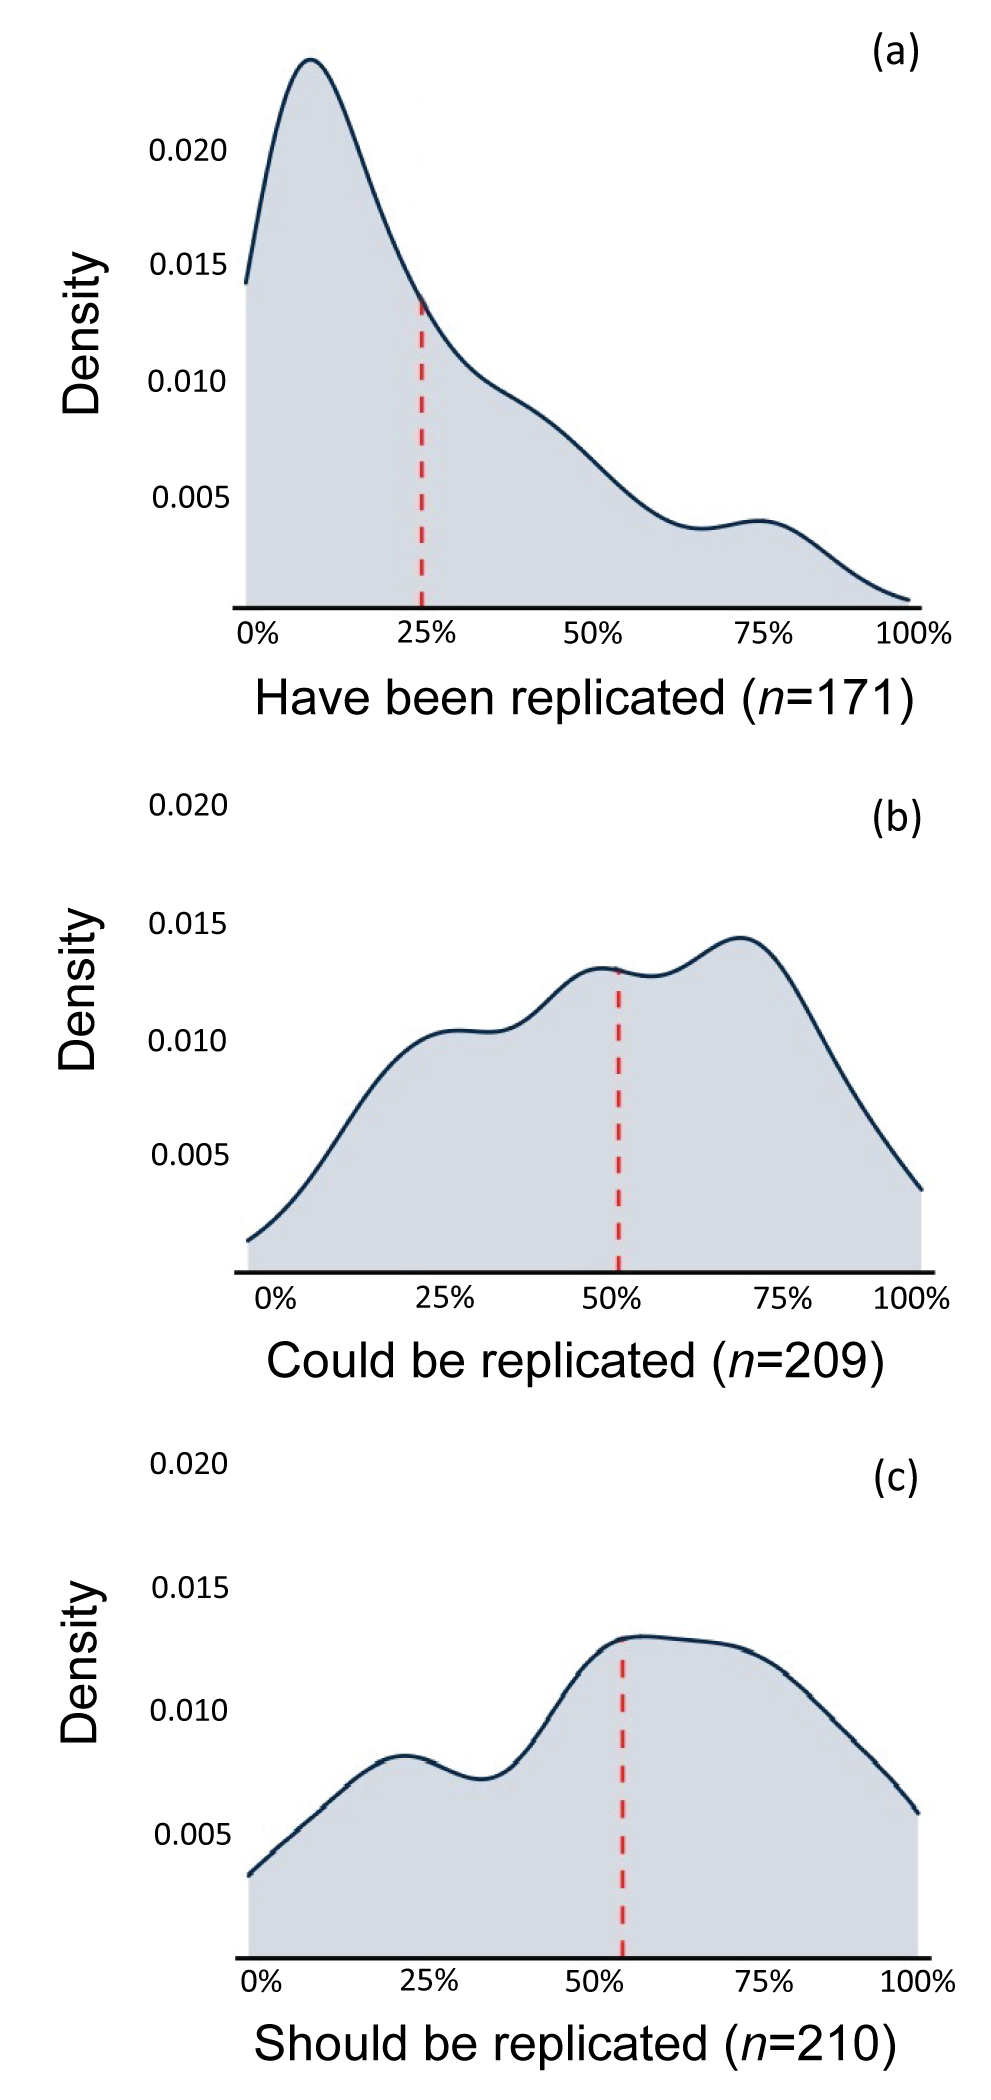
\includegraphics[scale=0.5]{results/figures/Fig-Q12-HCS.png}
    \caption{Estimates of the percentage of geographic studies that (a) have been replicated, (b) could be replicated, or (c) should be replicated}
    \label{fig:Q12-HCS}
\end{figure}

%%%%%%%%%%%%%%%%%%%%
\newpage

\begin{figure}[hbt!]
    \centering
    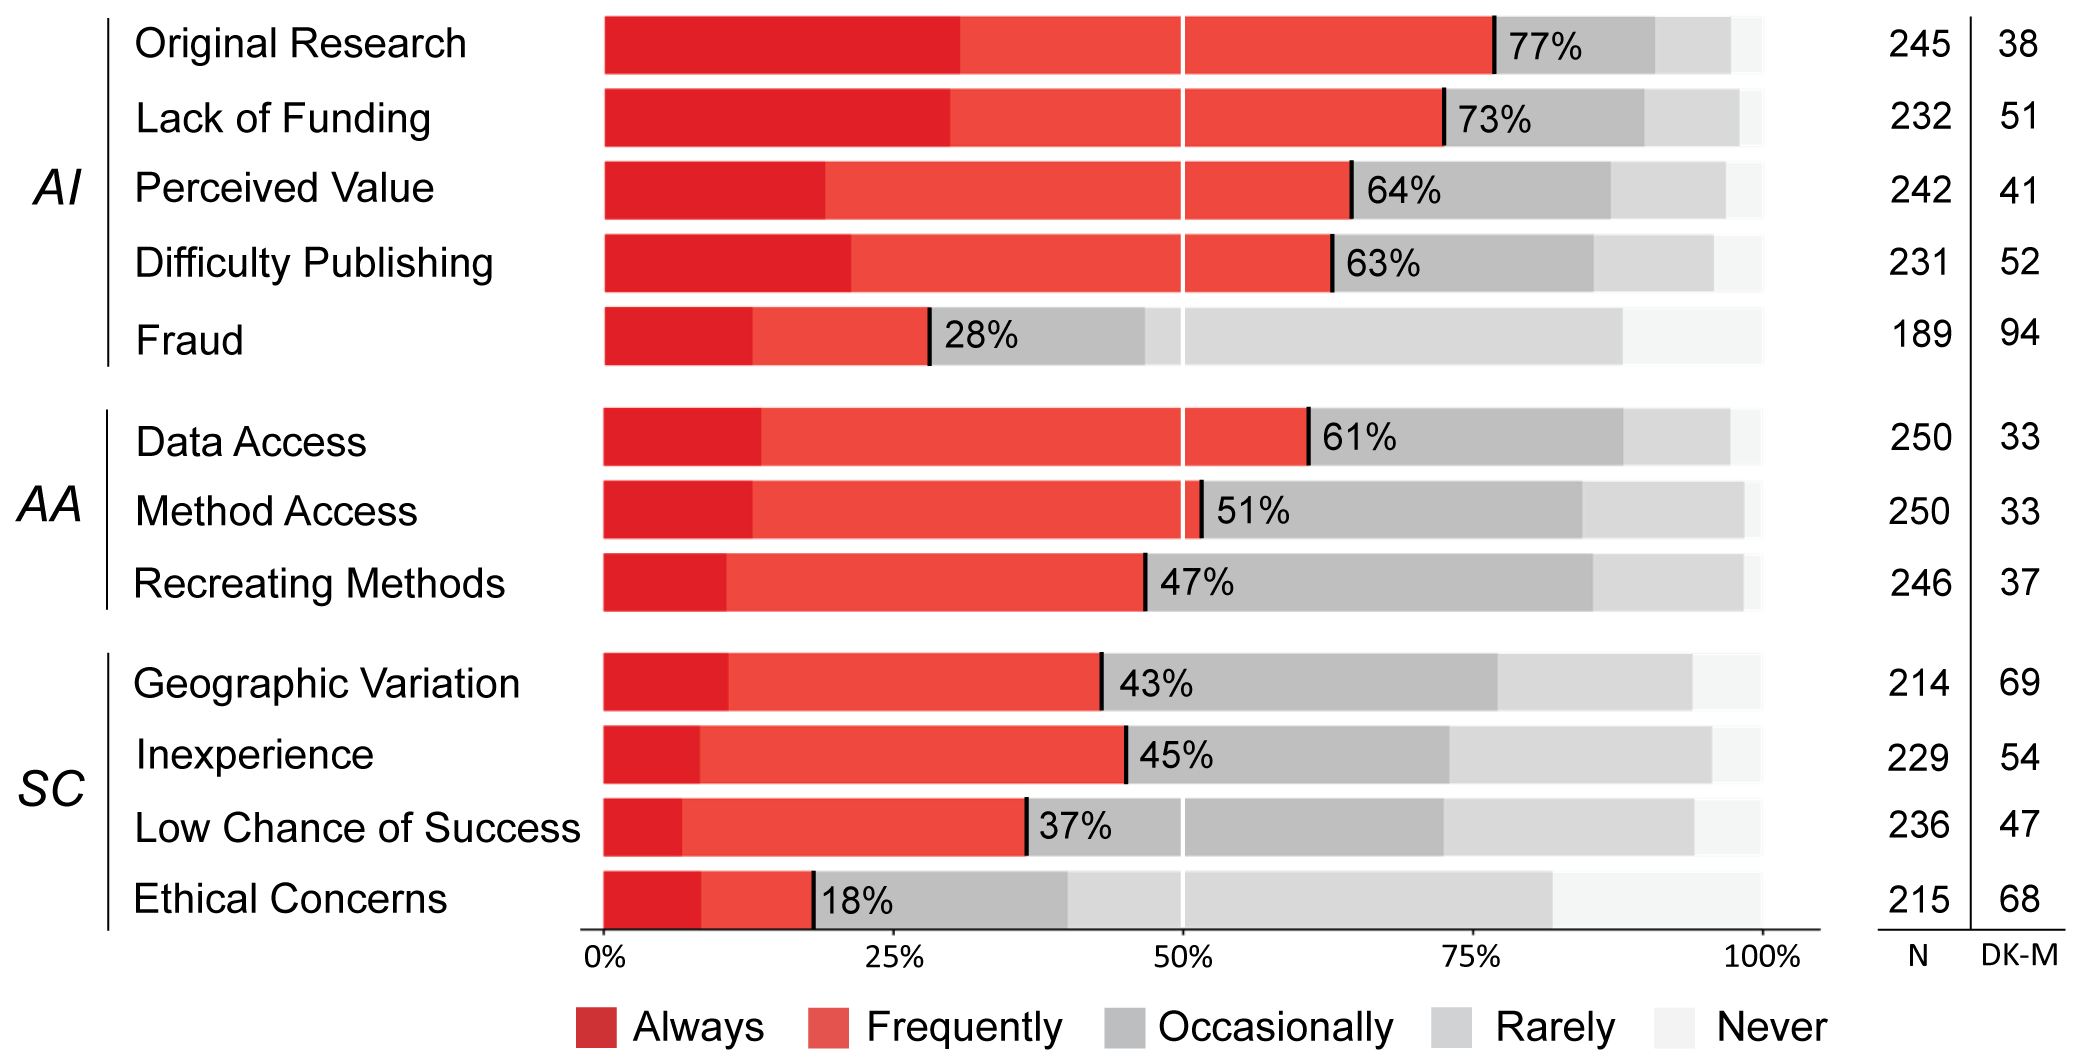
\includegraphics[scale=0.80]{results/figures/Fig-Q15-Decisions.png}
    \caption{Factors Affecting Researcher Decisions to Undertake Replication Studies. Factors grouped by: Academic Incentives (AA), Artifact Accessibility (AA), Study Characteristics (SC).}
    \label{fig:Q15-DecisionFactors}
\end{figure}

%%%%%%%%%%%%%%%%%%%%
\newpage
\noindent PETER KEDRON is an Associate Professor in the School of Geographical Science and Urban Planning and core faculty member in the Spatial Analysis Research Center (SPARC) at Arizona State University, Tempe, AZ, 85283, US. Email: Peter.Kedron@asu.edu. His research interests include spatial analysis, geographic information science, economic geography, and the accumulation of knowledge about geographic phenomena. \\  
  
\noindent JOSEPH HOLLER is an Assistant Professor of Geography at Middlebury College, Middlebury, VT, 05753, US. Email: \\
  
\noindent SARAH BARDIN is a PhD candidate ...

\end{document}